\documentclass[a4paper]{article}
%\usepackage{amsfonts}
\usepackage{amsmath}
%\usepackage{amsthm}
\usepackage[utf8]{inputenc}
%\usepackage{hyperref}
\usepackage{booktabs}
\usepackage{graphicx}
\usepackage{subfig}
\graphicspath{{fig/}}

\title{Exercises on physical design}
\author{Rodrigo Arias Mallo}
\date{\today}

\newcommand*\mat[1]{ \begin{pmatrix} #1 \end{pmatrix}}
\newcommand*\arr[1]{ \begin{bmatrix} #1 \end{bmatrix}}
\newcommand*\V[1]{ \boldsymbol{#1}}

\begin{document}
\maketitle

\section{Exercise 5}

\subsection{Draw the initial network}
%
\begin{center}
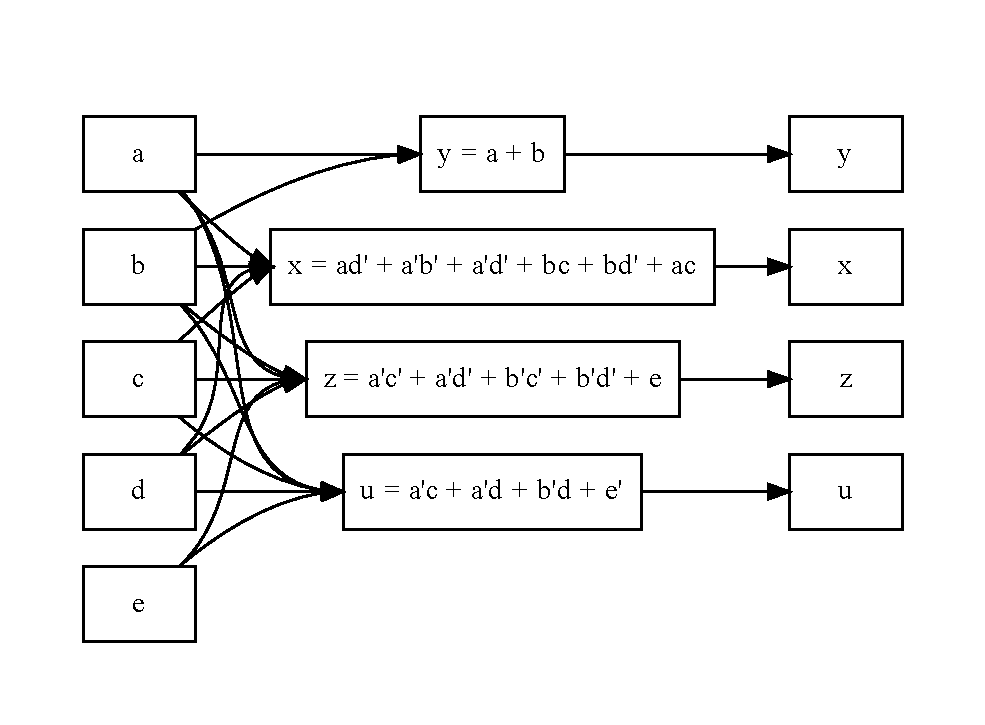
\includegraphics[scale=.5]{5a-graph.pdf}
\end{center}
%
\subsection{Algebraic division}
%
In order to perform the algebraic division $f_x / f_y$ we will apply the 
algorithm WEAK\_DIV described in the figure 10.9 of \cite{hachtel}. The 
functions are defined as
%
$$ f_x = ad' + a'b' + a'd' + bc + bd' + ac \quad f_y = a + b $$
%
With $F=f_x$ and $P=f_y$ we first compute $V^a$ as the set of cubes of $F$ that 
contain the literal $a$, with $a$ removed, giving $V^a = \{d', c\}$. The same 
for $b$, giving $V^b = \{d', c\}$. Then we compute $Q$ as the intersection and 
we get the same $Q = V^a \cap V^b = \{d', c\} = d' + c$. Finally with $PQ = (a + 
b)(c + d') = ac + ad' + bc + bd'$ we compute the rest as $R = F - PQ = a'b' + a' 
d'$ . So we can confirm that $F = PQ + R$. After substitution we have the 
following graph.
\begin{center}
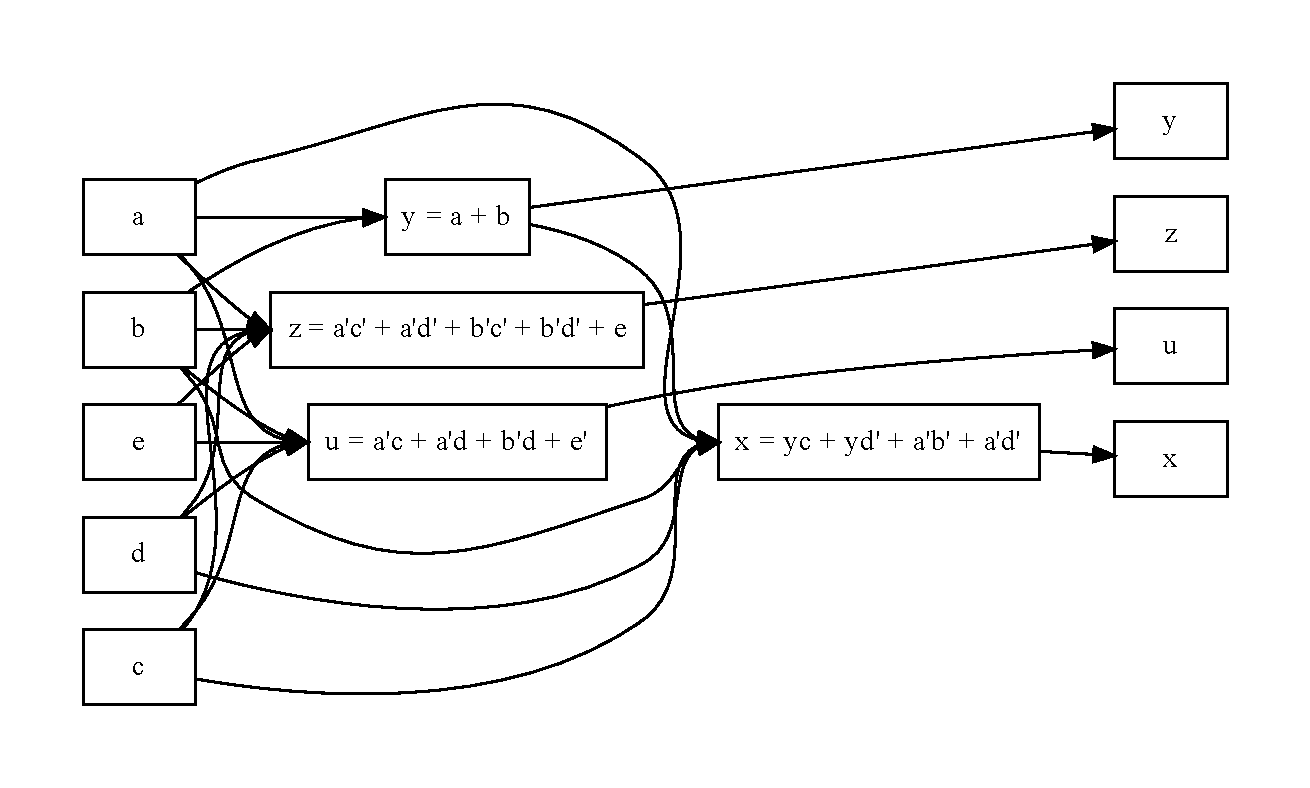
\includegraphics[scale=.5]{5b-graph.pdf}
\end{center}
%
\subsection{Kernels and co-kernels}
%
After trying both algorithms R\_KERNELS and KERNELS (8.3.3 and 8.3.4) in 
\cite{micheli}, I found it very complicated to work by hand. So I switched to 
the method of the cube insertion table, described in section 10.5.1 of 
\cite{hachtel}.
%
For $f_z = a'c' + a'd' + b'c' + b'd' + e$, let $n$ be the number of cubes, we 
first compute the co-kernels of level 0 by building the following table, placing 
the first $n-1$ cubes in columns, and the last $n-1$ cubes in columns.
%
\begin{center}
\begin{tabular}{c|cccc}
%\toprule
			 &  $a'c'$   &   $a'd'$   &   $b'c'$   &   $b'd'$  \\
\hline
%\midrule
$a'd'$ &  $a'$     &            &            &           \\
$b'c'$ &  $c'$     &      0     &            &           \\
$b'd'$ &  $0$      &     $d'$   &    $b'$    &           \\
$e$    &   0       &      0     &     0      &     0     \\
%\bottomrule
\end{tabular}
\end{center}
%
Then, we compute the intersection of the cubes pairwise. Cells above the 
diagonal are not needed. As we didn't discover co-kernels with more than one 
literal, we know that there are no co-kernels in the next levels. So we finally 
get $C(f_z) = \{a', b', c', d', 1\}$. Now, to compute the kernels, we can 
iterate for each co-kernel, and divide $f_z$ by each one, and the quotient would 
be the respective kernel. So we easily see that %
$K(f_z) = \{a' + b', c' + d', f_z\}$

For the function $f_u = a'c + a'd + b'd + e'$ we proceed in a similar way 
building the table.
%
\begin{center}
\begin{tabular}{c|ccc}
%\toprule
			 &  $a'c'$   &   $a'd'$   &   $b'd$   \\
\hline
%\midrule
$a'd'$ &   $a'$    &            &           \\
$b'd$  &    0      &     $d$    &           \\
$e'$   &    0      &     0      &    0      \\
%\bottomrule
\end{tabular}
\end{center}
%
And as before, we finish the procedure at level 0 as we didn't find co-kernels 
of more than one literal. We have $C(f_u) = \{a', d, 1\}$, and from there we 
build the associate kernels $K(f_u) = \{a'+b', c+d, f_u\}$
%
\subsection{Multi-cube extraction}
%
Once we have the kernels of both functions, we can extract a multi-cube common 
subexpression, in order to simplify the logic network. After factoring $z$ and 
$u$ we have
%
$$ z = (a' + b')(c' + d') + e \quad  u = d(a' + b') + a'c + e'$$
%
Which is decomposed into $ w = a'+b'$, $v = c'+d'$ and $ z = wv+e $. And for $u$ 
we have $p = a'+b'$ and $u = dp + a'c + e'$. We see that $w = p$ so we can 
replace $p$ by $w$ in $u$, giving $u = dw + a'c + e'$.
%
% TODO: Write the end by describing the elimination process



\newpage

\bibliography{biblio}
\bibliographystyle{ieeetr}

\end{document}
